\section{Feature detection and contributing factors}  \label{sec:features}

\begin{figure}[t]
    \centering
    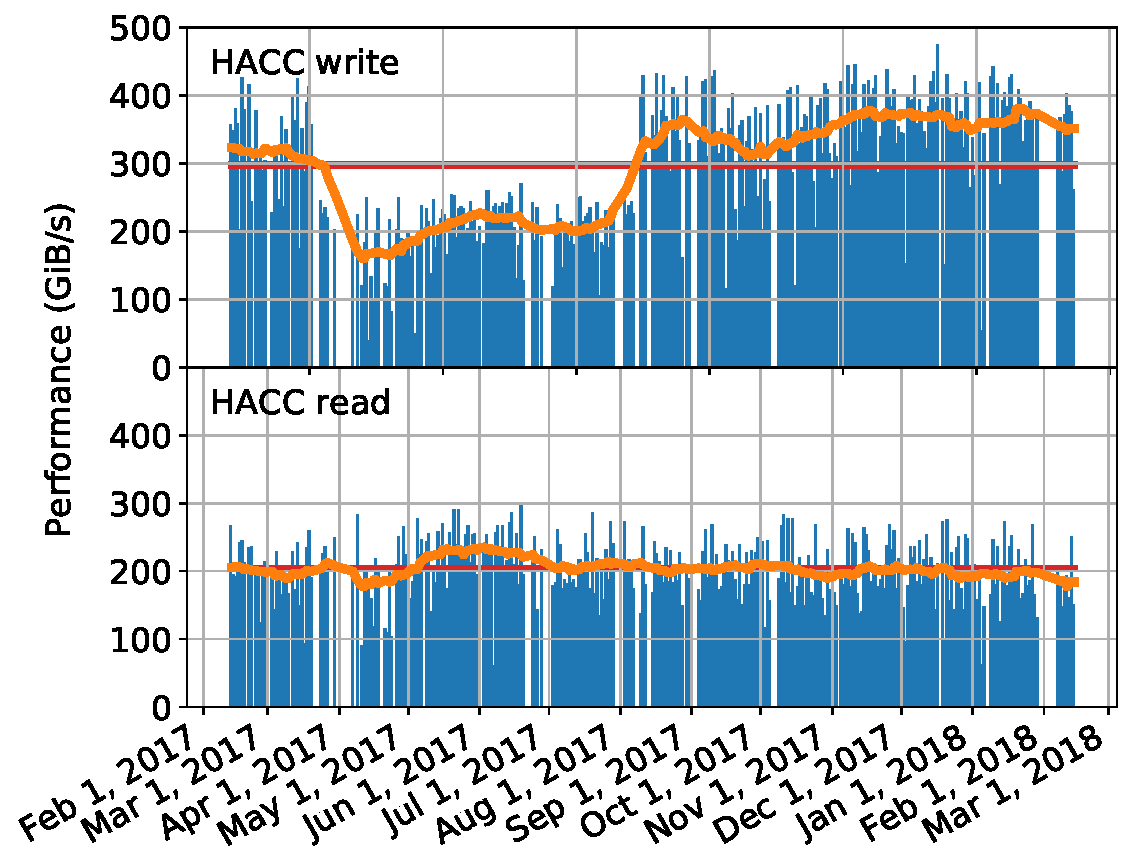
\includegraphics[width=1.0\columnwidth]{timeseries_baseline-cscratch_hacc_io_read_fpp_read}
    \vspace{-.35in}
    \caption{Performance evolution of HACC file-per-process  workload on Cori.  Red line is the overall mean (298 GiB/sec write, 204 GiB/sec read), orange line is 28-day SMA, and blue bars are daily performance measurements.}
    \label{fig:timeseries_baseline}
%   \vspace{-.3in}
% UP01 to UP03 upgrade, UP03 to UP04
\end{figure}\

As shown in Figure \ref{fig:summary-heatmap}, I/O performance variation is not randomly distributed.  To quantify such time-dependent performance variation, we propose applying simple moving averages (SMAs) as a means to identify correlated performance trends in production parallel file systems.
Given a time window of width $w$, we define the SMA for a metric $M$ at time $t$ as the average value of $M$ over $-0.5w <= t < +0.5w$;
when chosen to be sufficiently wide (e.g., $w = 28$ days) with respect to the benchmark frequency (nominally one day), the SMA distinguishes long-term performance variation (such as that caused by degraded file system health) from high-frequency variation caused by transient sources (such as conflicting jobs and network congestion).

\subsection{Longer-term behavior} \label{sec:features/longterm}

\TODO{How do we identify cases where performance is diverging in a
significant, sustained way?  Slowly worse, worse at at once, improving etc.}

\TODO{Once we've found these regions, how do we then find the factors that
contributed to that behavior?}

The 28-day SMA is for the HACC workload on Cori shown in Figure \ref{fig:timeseries_baseline} and highlights an example of long-term performance variation in the write workload:

\begin{enumerate}
\item The nominal performance of specific applications' I/O can vary over the service life of a storage system and its dependent components with periods of variation extending for months at a time
\item Not all workloads are affected by such long-term variation equally; in the case of HACC on Cori, write performance was adversely affected by a specific Lustre patch, while read performance of that same application was unaffected.
\end{enumerate}

Thus, it is important to contextualize I/O performance variation within the longer-term performance state of each storage subsystem to clarify whether the observation of "poor performance" is poor with respect to a longer-term performance depression or poor in the absolute capability of the storage system.

To provide this time-dependent context, we can use a second SMA with a longer window $w$ to compare the variation of the shorter-term performance with a more stable, long-term representation.  Figure \ref{fig:timeseries_baseline} includes the extreme case where ${w \rightarrow \infty}$ (i.e., the mean performance over the entire year) and, in the case of HACC write performance, visibly distinguishes the extent of the long-term performance depression that occurred between April and August.

Finding the intersection points between these two SMAs also provides an analytical tool for demarcating \textbf{performance regions};
for example, the intersection between $\textup{SMA}_{28}$ and $\textup{SMA}_\infty$ in Figure \ref{fig:timeseries_baseline} occurs at March 23 and August 8.
By comparing these dates to the service history of Cori, this performance depression was retrospectively attributed to patches applied to the Lustre clients on Cori on March 24 and August 10--within two days of the SMA interception points.







\subsection{Transitions between performance regions} \label{sec:features/transitions}

\begin{figure}[t]
    \centering
    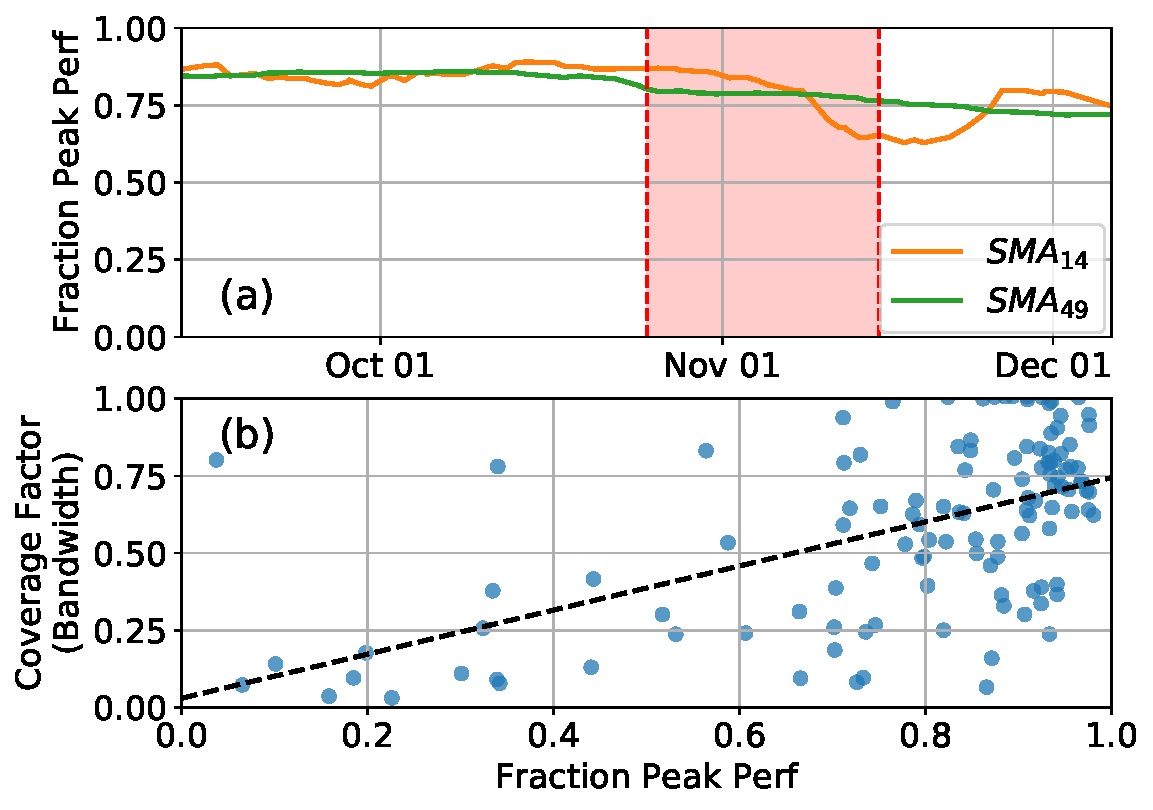
\includegraphics[width=1.0\columnwidth]{mira-correlation-region}
    \vspace{-.35in}
    \caption{Correlation between performance and $CF_{bw}$ in a transition between performance regions on Mira. (a) shows a region automatically detected using the centroid method, and (b) shows the correlation between performance and $CF_{bw}$ in that region.  Correlation coefficient is $0.565$ and p-value is ${1.48 \times 10^{-11}}$; dashed line in (b) is a linear fit with slope $0.714$ drawn for visual aid.}
    \label{fig:mira-correlation-region}
%   \vspace{-.3in}
% UP01 to UP03 upgrade, UP03 to UP04
\end{figure}

Long-term behavior has very low frequency by definition, so analyzing the causes of a few long-term performance depressions by hand (as was done in characterizing the HACC write performance in Figure \ref{fig:timeseries_baseline}) remains tractable.
However with sufficiently high observation frequency and comprehensive monitoring throughout the I/O subsystem, it is possible to both identify and characterize contributors to these long-term performance depressions.

Performance can be effectively correlated to with other metrics collected during the duration of each I/O-intensive job if (1) a sufficient numbers of jobs ran within that region to establish statistical confidence, and (2) there is sufficient variation observed in a region of interest.
To identify performance regions of sufficient width to satisfy (1), we generalize the approach taken to identify longer-term behavior in Section \ref{sec:features/longterm} and define $\textup{SMA}_{long}$ and $\textup{SMA}_{short}$ as simple moving averages with differing window lengths.
Adjusting $w_{short}$ and $w_{long}$ allows this approach to partition performance data into regions that capture sufficient measurements for confident correlations to be calculated.
To prevent the creation of very short performance regions, we also discard all intersection points that would generate a region with fewer than seven observations.

To satisfy (2) and capture regions that exhibit a broad range of performance measurements, we first determine the centermost measurement in each region from (1) and define the data between these central values as \textbf{transition regions}.
For each such transition region bounded by times $t_0$ and $t_f$, we then discard those regions where

\begin{equation}
abs \left (
\frac
	{ \textup{SMA}_{short}(t=t_0) - \textup{SMA}_{short}(t=t_f) }
	{\textup{SMA}_{short}(t=t_f)}
\right ) < C
\end{equation}

and $C$ is a cutoff threshold typically between 0.15 and 0.40 whose optimal value is a function of $w_{short}$, $w_{long}$, and how variable the storage system performance tends to be over long periods of time.  Given a well-chosen $C$, the result set of transition regions satisfy both the (1) sampling criterion and (2) diversity criterion.

To demonstrate the utility of this approach, we apply it to the entirety of the fraction of peak performance observations from Mira.
With $C = 0.15$, only two transition regions were identified for the entire year.
For each region, we then calculated the Pearson correlation coefficient between the fraction peak performance measurements and all other telemetric data associated with each job.
Using a p-value threshold of ${1.0 \times 10^{-5}}$, only one of the two regions (shown in Figure \ref{fig:mira-correlation-region}a) exhibited significant correlation, and the bandwidth coverage factor was the only metric that showed strong (${R = 0.565}$) correlation with high confidence (Figure \ref{fig:mira-correlation-region}b).
While we cannot determine causation from this correlation, this transition region correlation analysis automatically identified a long-term performance transition between October 13 and November 15 that was strongly correlated with bandwidth contention.
Given that sustained performance degradation caused by bandwidth correlation (or any other factors) were not observed at any other time during the year on Mira, the contentious activity was likely not caused by routine job traffic and may have been related to year-end activity on the system.







\subsection{Shorter-term behavior} \label{sec:features/shortterm}

\begin{figure}[t]
    \centering
    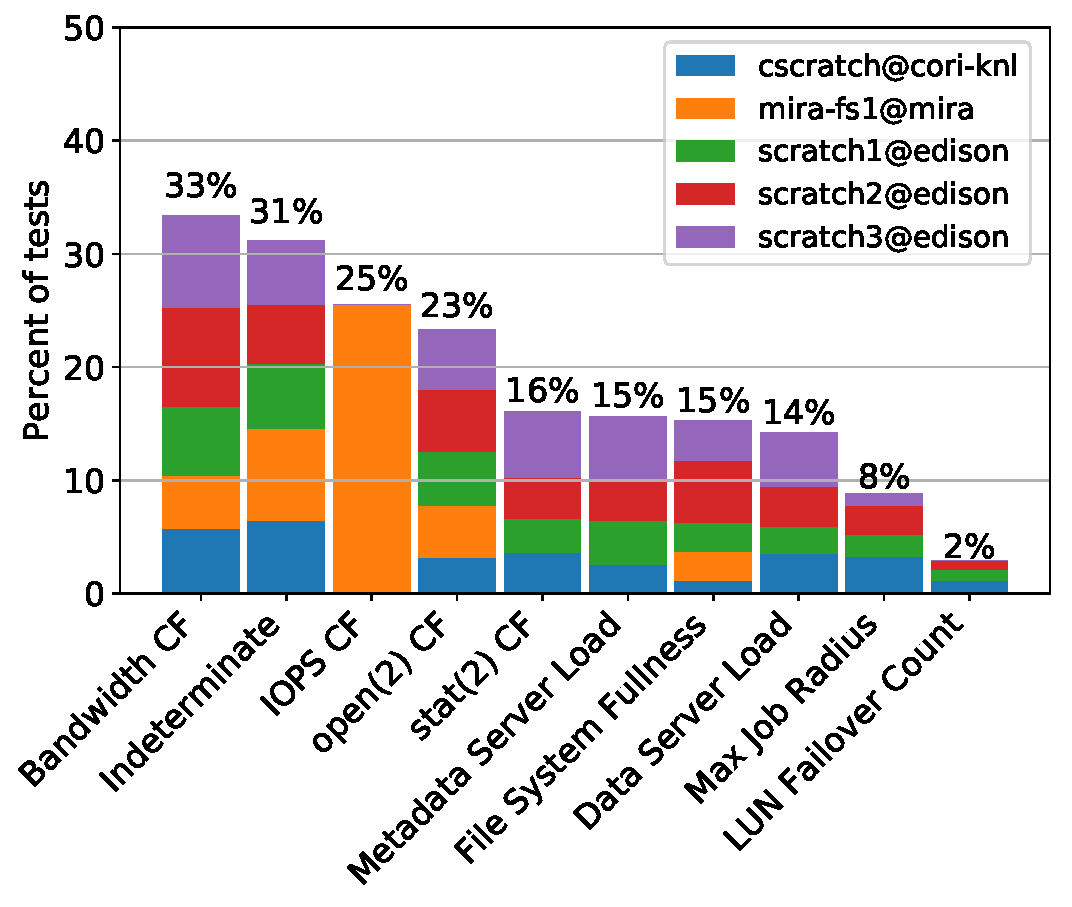
\includegraphics[width=1.0\columnwidth]{contributors-bad-by-system}
    \vspace{-.35in}
    \caption{Metrics that correlated with poor I/O performance across all file systems and benchmarks tested.  "CF" refers to coverage factor as defined earlier; "Indetermine" are those jobs where no metrics could be classified as contributors.
    \TODO{Shall we add some explanation for coverage factor as the reviewers may not be familiar with UMAMI? --Teng}}
    \label{fig:contributors-bad-by-system}
%   \vspace{-.3in}
% UP01 to UP03 upgrade, UP03 to UP04
\end{figure}

\TODO{This is where we introduce methodology for flagging regions,
identifying key point, running umami, binning likely contributors, etc.}


\TODO{clean this up: In contrast, shorter-term variations in I/O performance are both more frequent and more perceptible by users, and automating the process of identifying those regions and the factors contributing to reduced performance is more urgent.

...}

To illustrate this latter point, we use SMAs to define \emph{performance regions} that can be analyzed using the UMAMI method~\cite{Lockwood2017} where the performance of a job of interest is visualized alongside a variety of metrics concurrently collected from component-level monitoring tools.
By focusing on particular jobs of interest \emph{and} the other jobs that also ran within the same performance region, we can contextualize both the application's I/O performance and the telemetric data collected during that job to identify factors that statistically correlate with abnormal performance.

...

We first separated each combination of five file systems, four test applications, and read/write character into a set of 40 performance measurements spanning a year.
Using $SMA_{short}$ of $w = 7$ days and $SMA_{long}$ of $w = 28$ days, we then partitioned each set of measurements into between 16 and 27 performance regions.
For each region, we then applied a classification method whereby
\TODO{A few sentences answering why 16 and 27 regions are generated may be helpful. May also replace 40 by 5$\times$4$\times$2 for easier understanding -Teng}
\begin{enumerate}
\item The lowest performance measurement of that region is identified as a Job of Interest
\item TOKIO's UMAMI analysis is performed where metrics that speak to application-side performance, file system load, file system health, system batch scheduler load, and system topology are all combined into a single holistic description of each job's I/O performance
\item The value of each metric measured during the Job of Interest is compared to the statistical distribution of those metrics across all other jobs in the performance region.  All metrics whose values were at their worst at the same time the Job of Interest was running are flagged as potential contributors to the poor performance of the job of interest.
\end{enumerate}

The result of this analysis is zero or more metrics being flagged as potential contributors to poor performance within each performance region for each application, file system, and read/write mode.

Aggregating all of the performance regions' poor-performance contributors yields a broad overview of the metrics that most commonly coincide with poor performance across all of the test systems.
This distribution, shown in Figure \ref{fig:contributors-bad-by-system}, reveals that abnormally high bandwidth contention was found to coincide with abnormally poor performance most frequently.

\TODO{Update Fig \ref{fig:contributors-bad-by-system} to use the new minmax classifier}

\TODO{Define the metrics in Fig \ref{fig:contributors-bad-by-system}}

\TODO{Somewhere, maybe not here, revisit findings from PDSW paper and see if
they still make sense in year long context?}
